\documentclass[a4paper,12pt]{article}
\usepackage[utf8]{inputenc} % Kodierung
\usepackage[T1]{fontenc} % Explizite Nennung des Fonts
\usepackage[ngerman]{babel} % Sprache
\usepackage{graphicx} % immer benötigt für das Einbinden von Graphiken
%\usepackage{blindtext} % Wenn man das Layout prüfen will, kann hier mit \blindtext Text eingfügt werden.
\usepackage{parskip} % Für den Abstand zwischen 2 Absätzen.
\setlength{\parskip}{12pt plus80pt minus10pt} % Genaue Einstellung von parskip
%\usepackage{easy-todo} % Mit \todo{} Todos einfügen
%\usepackage{csquotes} % Für ordentlichen Anführungszeichen
%\usepackage[iso, german]{isodate} % Für eine deutsche Formatierung des Abgabedatums / Eidesstattlicher Erkärung
\usepackage[style=numeric, backend=biber, sortlocale=de_DE, sorting=none]{biblatex} % Biber backend für Literaturverzeichnis
\addbibresource{literatur/bibliography.bib} % Einbinden der Literatur.
% \DeclareLanguageMapping{german}{german-apa} % Anpassen Spracheinstellungen im Literaturverzeichnis.
\usepackage[activate={true,nocompatibility},
	final,
	tracking=true,
	kerning=true,
	expansion=true,
	spacing=true,
	factor=1050,
	stretch=25,
	shrink=10]{microtype} % Für die Feineinstellung der Zeichensetzung.
\usepackage{booktabs}
\usepackage{appendix}
%\usepackage[rflt]{floatflt} % Das hat Opi auskommentiert (28-NOV-2021)
\usepackage{fancyvrb}
\usepackage[hidelinks]{hyperref} % Klickbare aber nicht markierte Links im PDF
\usepackage{url} % Klickbare aber nicht markierte Links im PDF
\usepackage[onehalfspacing]{setspace}
\usepackage{fancyhdr} % Für schönere Kopf-/Fußzeilen und Fußnoten.
\usepackage[right=2 cm, left=4 cm, top=2.5 cm, bottom=3 cm]{geometry} % Seitenränder
\usepackage{pbox}
%\usepackage{tabulary}
\usepackage{picinpar}
\usepackage{amsmath}
\usepackage{amssymb}
\usepackage{fleqn}
%\usepackage{equations} % Das hat Opi auskommentiert (28-NOV-2021)
\usepackage{verbatim} % Das hat Opi eingefügt (wegen \begin{comment} ... \end{comment}, 28-NOV-2021)
%\usepackage{showframe}

\sloppy
\fancyhf{}
\rfoot{\thepage}
\renewcommand{\headrulewidth}{0pt}
%Special cells with linebreaks possible
\newcommand{\specialcell}[2][c]{%
	\begin{tabular}[#1]{@{}t@{}}#2\end{tabular}}
%define blockquote-quotation environment
\renewenvironment{quotation}{
	\leftskip1cm
	\rightskip1cm
	\noindent
	\setstretch{1}
	\small
}

% define Footnote
\renewcommand\footnoterule{\kern-3pt \hrule width 3in height 0.7pt \hskip3pt \kern 2.6pt}
\let\oldfootnote\footnote
\renewcommand\footnote[1]{%
	\oldfootnote{\hspace{2mm}#1}}
%%%%%

% microtyping around some characters

%Extra-spacing around dash, and quotation-marks, and parentheses
\SetExtraKerning[unit=space]
	{
		encoding={*}, family={qhv}, series={b}, size={normalsize,large,Large}
	}
	{
		\textendash={400,400}, % for double-dash
		\textquotedblleft={ ,120}, % for left quotation-mark
		\textquotedblright={170, }, % for right quotation-mark
		"28={ ,250}, % left bracket, add space from right
		"29={300, } % right bracket, add space from left
	}

%%%%%


\makeatletter
\newcommand{\MSonehalfspacing}{%
  \setstretch{1.44}%  default
  \ifcase \@ptsize \relax % 10pt
    \setstretch {1.448}%
  \or % 11pt
    \setstretch {1.399}%
  \or % 12pt
    \setstretch {1.433}%
  \fi
}
\newcommand{\MSdoublespacing}{%
  \setstretch {1.92}%  default
  \ifcase \@ptsize \relax % 10pt
    \setstretch {1.936}%
  \or % 11pt
    \setstretch {1.866}%
  \or % 12pt
    \setstretch {1.902}%
  \fi
}
\newcommand{\MSverbatimspacing}{%
  \setstretch{1.44}%  default
  \ifcase \@ptsize \relax % 10pt
    \setstretch {1}%
  \or % 11pt
    \setstretch {1}%
  \or % 12pt
    \setstretch {1}%
  \fi
}
\makeatother
\begin{document}
\newgeometry{margin=2.5cm}
\begin{titlepage}
\thispagestyle{empty}
\newcommand{\HRule}{\rule{\linewidth}{0.5mm}}
\hspace{1cm}
\center

\textsc{\huge Besondere Lernleistung}\\[2.0cm]
\textsc{\Large Paulsen-Gymnasium}\\[0.8cm]
\textsc{\Large Berlin-Steglitz}\\[0.8cm]
\MSonehalfspacing

\HRule\\%[1.4cm]
\MSdoublespacing
{ \huge \bfseries Die Verbindung des \\
pythagoreischen Lehrsatzes mit dem Großen Fermatschen Satz unter Beachtung der historischen Entwicklung}\\[0.2cm]
\HRule \\[2.4cm]
\MSonehalfspacing

\raggedright
\item[{Name:}] Charlotte Specht
\item[{Betreuende Lehrkraft:}] Herr Wessel
\item[{Datum:}] 06.12.2021
\item[{Hauptfach:}] Mathematik
\item[{Bezugsfach:}] Geschichte

\end{titlepage}
\restoregeometry

\setstretch{1.9}
\microtypesetup{protrusion=false}
\tableofcontents
\microtypesetup{protrusion=true}
\thispagestyle{empty}

\MSonehalfspacing
\newpage
\pagestyle{fancy}
\setcounter{page}{3}

%\setcounter{page}{1}
\renewcommand{\figurename}{Abb.}
%\setlenght{\mathindent}{30pt}
\def\bdm{\begin{displaymath}}
\def\edm{\end{displaymath}}
\def\bdma{\begin{eqalignno*}}
\def\edma{\end{eqalignno*}}
\def\mkm{\mkern 1mu}
\def\mkmm{\mkern 2mu}
\def\mkmmm{\mkern 3mu}
\renewcommand{\baselinestretch}{1.5}
\small
\normalsize
\makeatletter
\newcommand*{\rom}[1]{\expandafter\@slowromancap\romannumeral #1@}
\makeatother

\section{Einleitung}

In dieser Besonderen Lernleistung (BLL) werde ich zunächst Pythagoras' Leben und den pythagoreischen Bund vorstellen. Danach werde ich den Satz des Pythagoras erläutern und klären, was ein mathematischer Beweis ist, um mehrere Beweise für den Satz des Pythagoras zu erläutern. Anschließend wird der zweite Teil der Arbeit von Fermat und seinem letzten Satz handeln, sowie dessen Verbindung zum pythagoreischen Lehrsatz und den langen Weg, bis Fermats letzter Satz von Andrew Wiles bewiesen werden konnte.

\section{Pythagoras von Samos} \label{einleitung}

\subsection{Pythagoras' Leben}

Pythagoras von Samos war ein bedeutender Mathematiker und Philosoph \cite{PythagorasWiki}. Er gilt als Begründer der Zahlentheorie, da er die Beziehungen zwischen Zahlen und deren Eigenschaften untersucht und so Muster in Zahlenfolgen entdeckt hat. Außerdem war er politisch aktiv, gründete einen politisch religiösen Bund und beschäftigte sich mit Astronomie.

Pythagoras selbst verfasste keine eigenen Schriften, weshalb alles, was sich über sein Leben sagen lässt, aus Mythen und Legenden stammt. Desweiteren ist es schwierig zu unterscheiden, welche Lehren von Pythagoras selbst stammen und welche von späteren Pythagoreern. Es ist auch unklar, ob sich Pythagoras überhaupt für Wissenschaft interessierte oder er doch nur der Anführer des Bundes war und sich nur die Pythagoreer:innen mit Wissenschaft beschäftigten.



 Pythagoras wurde ungefähr 580 v. Chr. \cite{PythagorasGeburt} als Sohn des Kaufmanns Mnesarchos und dessen Frau Pythais auf der griechischen Insel Samos im  Ägäischen Meer geboren \cite{PythagorasLeben}. Er wurde von dem Philosophen Pherekydes von Syros unterrichtet. Als junger Erwachsener begann er eine zwanzig Jahre lange Reise in verschiedene Länder, wie zum Beispiel Babylon, Persien, Ägypten und Phönizien \cite[S. 31-34]{Buch}. Dabei lernte er besonders von den Babyloniern und den Ägyptern viele mathematische Methoden kennen. Die Mathematik wurde zum Beispiel angewendet, um die Erde zu vermessen, doch sie waren nicht daran interessiert, ihre Erkenntnisse auch zu beweisen, denn damals war es vor allem wichtig, dass man sich darauf verlassen konnte, dass die Methoden in alltäglichen Situationen zu richtigen Ergebnissen führten.

Als Pythagoras nach seiner langen Reise zu seiner Heimatinsel zurückkehrte, herrschte dort der Tyrann Polycrates, der Pythagoras anbot, an seinem Hof zu arbeiten. Doch Pythagoras erkannte, dass dieses Angebot nur eine Falle war, um ihn mit seinen eigenen philosophischen Ideen unter Kontrolle zu halten, und lehnte das Angebot ab. Stattdessen lebte er alleine in einer Höhle am Rand der Insel und konnte sich dort ohne Angst vor dem Tyrannen mathematischen Problemen und philosophischen Ideen widmen. Da er sehr einsam war, jedoch viel Wissen hatte, wünschte er sich einen Schüler, dem er all sein Wissen beibringen konnte. Deshalb bestach er einen Jungen, sein erster Schüler zu werden. Der Junge begeisterte sich immer mehr für den Unterricht, sodass er bald kein Geld mehr von Pythagoras für die Lektionen verlangte.

532 v. Chr. musste Pythagoras aufgrund seiner philosophischen Ansichten von seiner Heimatinsel fliehen. Er floh mit seinem Schüler und seiner Mutter in die Stadt Kroton, die in der süditalienischen Kolonie Magna Graecia lag. Dort traf er auf den wohlhabenden Mathematiker und Philosoph Milon, der seine Forschungen finanziell unterstützte und Pythagoras Platz zum Wohnen und Lehren zur Verfügung stellte.

Nach seiner Ankunft gründete Pythagoras in Kroton den \emph{pythagoreischen Bund}. Dies war eine Schule, in der er den später 600 Mitgliedern seine Lehren beibrachte. Seine Schüler:innen konnten auch eigene Lehren formulieren und es entstand ein religiöser Bund. Die Mitglieder des pythagoreischen Bundes lösten mathematische Probleme, um die Geheimnisse des Universums zu ergründen und den Göttern näher zu kommen. Sie hatten eine neue Weltanschauung, die den philosophischen Ansichten Pythagoras' entsprach. Dieser Bund ist vergleichbar mit einer Sekte, in der Pythagoras der Sektenführer war, denn die Mitglieder mussten alles, was sie besaßen, in einen Gemeinschaftsfonds geben und beim Eintritt einen Schwur ablegen, dass sie die neuen Entdeckungen des Bundes nicht außerhalb des Bundes verbreiten. Wenn sie sich nicht daran hielten, wurden sie hart bestraft. Außerdem lebten die Pythagoreer:innen nach der pythagoreischen Art des Lebens, die besagte, dass man diszipliniert und bescheiden leben solle und dem Bund treu bleiben müsse.

Bei der 76. Olympiade, die ca. 510 v. Chr. stattfand, gab es einen Aufstand in Sybaris \cite[S. 50-52]{Buch}. Die alte Regierung wurde gestürzt und seitdem herrschte dort der Tyrann Telys. Die alten Regierungsmitglieder flohen in die nahe gelegene Stadt Kroton, wo Milon und Pythagoras lebten. Telys und seine Anhänger:innen forderten die Auslieferung der geflüchteten ehemaligen Regierungsmitgliedern, um sie für ihre Taten in Sybaris zu bestrafen, doch Milon und Pythagoras forderten die Krotoner:innen auf, die Flüchtlinge zu schützen. Daraufhin griff Telys' Armee, die aus 300$\mkmmm$000 Soldaten bestand, Kroton an. Die Krotoner stellten zur Verteidigung ihrer Stadt eine Armee mit 100$\mkmmm$000 Bürgern auf. So begann ein 70 Tage langer Krieg zwischen Sybaris und Kroton. Am Ende siegten die Krotoner unter Milons Führung und leiteten den Fluss Crathis um, mit dem Ziel Sybaris zu überschwemmen und zu zerstören.

In Kroton entstand ein Streit um die Kriegsbeute, denn die Bäuerinnen und Bauern sowie die Bürger:innen befürchten, dass der mittlerweile sehr mächtige pythagoreische Bund die gesamte Kriegsbeute für sich beanspruchen und zum Beispiel das neue Land nicht fair aufgeteilt werden würde. Neben ihrer Angst baute sich auch immer mehr Ärger gegenüber dem pythagoreischen Bund auf, da die Mitglieder ihre Entdeckungen nicht mit dem Volk teilten.

Kylon, ein Mathematiker und Philosoph, der in den pythagoreischen Bund aufgenommen werden wollte, jedoch abgelehnt wurde, da er aus Pythagoras' Sicht nicht gut genug war, nutzte die Angst und den Ärger des Volkes aus, indem er deren Abneigung und Neid gegenüber dem pythagoreischen Bund verstärkte. Er rief die Krotoner:innen dazu auf, die Schule des Bundes zu stürmen. Kylons Anhänger:innen umstellten Milons Haus und zündeten es an.

Bis zu diesem Punkt in der Geschichte sind sich die meisten Historiker:innen einig, doch was danach geschah, ist umstritten.

Die Einen sind der Meinung, dass Milon aus dem Haus fliehen konnte und überlebte, doch Pythagoras und viele seiner Schüler:innen in den Flammen starben. Die Schüler:innen, die fliehen konnten, wurden verfolgt und zerstreuten sich. Da Pythagoras tot war und so der pythagoreische Bund keine große Bedeutung mehr hatte, wurde es möglich, ihre Lehren zu verbreiten.

Die Anderen vermuten, dass Pythagoras vor der gewalttätigen Auseinandersetzung aufgrund der Unruhen in Kroton nach Metapontion floh und dort erst 480 v. Chr. starb. 

\subsection{Die Entdeckungen des pythagoreischen Bundes}

Die Entdeckungen des pythagoreischen Bundes basieren alle auf der Idee, dass es nur rationale Zahlen gibt, also Zahlen, die sich als Bruch ganzer Zahlen darstellen lassen. Im Folgenden werde ich einige dieser Entdeckungen vorstellen \cite[S. 37-41]{Buch}.

Die Pythagoreer:innen suchten zum Beispiel besondere natürliche Zahlen: die \emph{vollkommenen Zahlen}. Ob eine Zahl vollkommen ist, hängt von ihren Teilern ab. Die Pythagoreer:innen teilten die natürlichen Zahlen in \emph{abundante}, \emph{vollkommene} und \emph{defiziente} Zahlen ein (siehe Anhang 5.3). Sie fanden vollkommene Zahlen, wie die $6$, die $28$ und die $496$. Dabei entdeckten sie, dass alle vollkommenen Zahlen Summen aufeinander folgender natürlicher Zahlen, sogenannte \emph{Dreieckszahlen} (beginnend mit $1$), sind, wie man an diesen beiden Beispielen gut erkennen kann:
\begin{comment}
\vspace*{-0.75cm}
\hspace*{1.5cm}
\begin{minipage}{10cm}
  \begin{flalign*}
    &1 + 2 + 3 = 6,&\\
    &1 + 2 + 3 + 4 + 5 + 6 + 7 = 28,&\\
    &1 + 2 + 3 ... + 31 = 496.&\\
  \end{flalign*}
\end{minipage}
\vspace*{-0.75cm}
\end{comment}
\begin{align*}
1 + 2 + 3 &= 6,\\
1 + 2 + 3 + ... + 7 &= 28,\\
1 + 2 + 3 + ... + 31 &= 496.
\end{align*}

Des Weiteren untersuchte Pythagoras die Harmonie verschiedener Töne mit einer Leier. Er entdeckte, dass, damit zwei Töne harmonieren, die Frequenzen der Töne in einfachen Zahlenverhältnissen zueinander liegen müssen. Zum Beispiel klingt eine Quinte ($3:2$) oder eine große Terz ($5:4$) harmonisch.

Pythagoras' Schüler Hippasus untersuchte, wie man $\sqrt{2}$ als Dezimalzahl darstellen kann und entdeckte, dass diese Zahl nicht als Bruch ganzer Zahlen darstellbar ist. Somit ist $\sqrt{2}$ keine rationale, sondern eine irrationale Zahl. Seine neue Entdeckung stellte er Pythagoras vor, doch Pythagoras wollte nicht wahrhaben, dass es auch irrationale Zahlen gibt und ließ den Schüler daraufhin ertränken.

\subsection{Der Satz des Pythagoras}

\begin{figwindow}[0,r,{\vbox{\vskip-1mm \hbox{\hskip10mm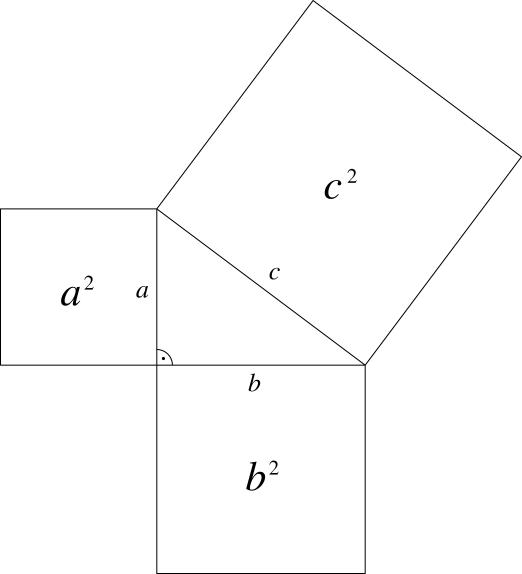
\includegraphics[width=60mm]{SatzDesPythagoras.jpg}}}},{Rechtwinkliges Dreieck}]
Pythagoras' bekanntester Satz ist heute unter den Namen ,,Satz des Pythagoras'' oder ,,Hypotenusensatz'' bekannt und besagt, dass in einem rechtwinkligen Dreieck das Quadrat über der Hypotenuse (hier Seite $c$) gleich der Summe der Quadrate über den beiden Katheten (hier Seite $a$ und $b$) ist (siehe Abb. 1). Die Gleichung lautet also mathematisch:

\vspace*{-0.75cm}
\hspace*{1.5cm}
\begin{minipage}{10cm}
  \begin{flalign*}
    a^{2} + b^{2} &= c^{2}.&\\
  \end{flalign*}
\end{minipage}
\vspace*{-0.75cm}

\end{figwindow}

Zum Beispiel erhält man mit $a = 3$ und $b = 4$ das Ergebnis $c = \sqrt{a^2 + b^2} = 5$.

Man kann also durch den Satz des Pythagoras die Länge einer beliebigen Seite in einem rechtwinkligen Dreieck berechnen, wenn die anderen beiden Seitenlängen gegeben sind.

Der Satz des Pythagoras ist reversibel \cite[S. 42,43]{Buch}. Das bedeutet, dass der Satz umkehrbar ist. Wenn also $a^{2} + b^{2} = c^{2}$ gilt, dann ist das Dreieck mit diesen Seitenlängen auf jeden Fall rechtwinklig. Der rechte Winkel liegt dann immer gegenüber der Hypotenuse $c$.

Der Kosinussatz stellt eine Verallgemeinerung des pythagoreischen Lehrsatzes dar und besagt, dass in einem beliebigen Dreieck folgende Gleichung gilt:

\vspace*{-0.75cm}
\hspace*{1.5cm}
\begin{minipage}{10cm}
  \begin{flalign*}
    c^2 &= a^2 + b^2 - 2ab\cdot \cos{(\gamma)}.\\
  \end{flalign*}
\end{minipage}
\vspace*{-0.75cm}

In einem rechtwinkligen Dreieck ist der der Seite c gegenüberliegende Winkel $\gamma = 90^\circ$ und damit $\cos{(90^\circ)} = 0$.

Dann gilt:

\vspace*{-0.75cm}
\hspace*{1.5cm}
\begin{minipage}{10cm}
  \begin{flalign*}
    c^2 &= a^2 + b^2.\\
  \end{flalign*}
\end{minipage}
\vspace*{-0.75cm}

Also ist der Satz des Pythagoras ein besonderer Fall des Kosinussatzes.

Die Beziehung zwischen den Seitenlängen in einem rechtwinkligen Dreieck wurde wahrscheinlich schon ungefähr 1000 Jahre vor Pythagoras von den Chinesen und Babyloniern entdeckt, doch der Erste, der einen Beweis für diesen Satz entdeckte, war Pythagoras. Man kann nicht ausschließen, dass es auch schon Beweise vor Pythagoras gab, doch die Chinesen und Babylonier waren mehr an der praktischen Anwendung interessiert als an Beweisen.

Mittlerweile gibt es sehr viele Beweise für den Satz des Pythagoras, von denen ich im Folgenden ein paar vorstellen werde, doch vorerst werde ich klären, was ein mathematischer Beweis ist.

\subsection{Was ist ein mathematischer Beweis?}

Bei einem Beweis wird versucht, mit der Hilfe von Argumenten glaubhaft zu machen, dass eine Aussage wirklich wahr ist. Man muss hierbei aber zwischen einem naturwissenschaftlichen Beweis und einem mathematischen Beweis unterscheiden \cite[S. 44-50]{Buch}. Bei einem naturwissenschaftlichen Beweis werden Hypothesen durch Experimente belegt oder eben widerlegt. Die Schlussfolgerung, ob die Hypothese wahr oder falsch ist, ist aber nicht zu 100 Prozent sicher. Vielleicht gibt es noch eine Situation, in der die Hypothese nicht wahr ist, denn man kann nicht jeden denkbaren Versuchsaufbau testen, gerade wenn die Anzahl der Möglichkeiten ins Unendliche geht. Diese trotzdem ziemlich hohe Wahrscheinlichkeit dafür, dass eine These wahr ist, reicht für die naturwissenschaftlichen Zwecke in der Regel aus, doch in der Mathematik ist das anders. Denn auf einem Beweis bauen oft viele andere Beweise auf. Das bedeutet, dass, wenn in einem der Beweise in dieser Kette von Beweisen ein Fehler ist, die darauf folgenden Beweise möglicherweise auch Fehler enthalten. Deshalb ist es bei mathematischen Beweisen wichtig, dass diese  allgemeingültig wahr sind.

Für einen mathematischen Beweis benötigt man ein oder mehrere \emph{Axiome} \cite{Beweise}. Das sind Aussagen, die entweder eindeutig wahr sind oder die schon bewiesen sind. Durch einen darauf folgenden logischen Gedankengang ist die Schlussfolgerung zu 100 Prozent wahr. So ist ein neuer \emph{Satz (Theorem)} entstanden. Im Folgenden werde ich mehrere Beweise für den Satz des Pythagoras vorstellen.

\newpage
\section{Beweise für den Satz des Pythagoras}

\subsection{Beweis mit Vektoren}

\begin{figwindow}[0,r,{\vbox{\vskip-1mm \hbox{\hskip10mm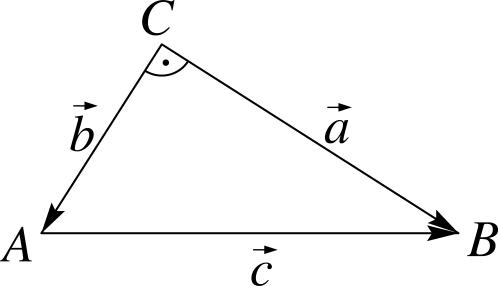
\includegraphics[width=60mm]{Vektoren.jpg}}}},{Beweis mit Vektoren}]

Das rechtwinklige Dreieck wird mit den Vektoren $\vec{a}$, $\vec{b}$ und $\vec{c}$ darstellt (siehe Abb. 2) \cite{BeweisVektoren}. Das Skalarprodukt $\vec{a} \cdot \vec{b} = 0$, da die beiden Vektoren $\vec{a}$ und $\vec{b}$ aufgrund des rechten Winkels senkrecht zueinander stehen.

\end{figwindow}

Den Vektor $\vec{c}$ kann man auch als Linearkombination der Vektoren $\vec{a}$ und $\vec{b}$ darstellen:
\begin{comment}
\vspace*{-0.75cm}
\hspace*{1.5cm}
\begin{minipage}{10cm}
  \begin{flalign*}
    \vec{c} = \vec{a} - \vec{b}.\\
  \end{flalign*}
\end{minipage}
\vspace*{-0.75cm}
\end{comment}
\begin{align*}
\vec{c} &= \vec{a} - \vec{b}.
\end{align*}
Das bedeutet, dass folgende Gleichungen gelten:
\begin{align*}
\vec{c}^{\:2} &= (\vec{a} - \vec{b})^2, \\
&= \vec{a}^{\:2} - 2\mkm\vec{a} \cdot \vec{b} + \vec{b}^{\:2}, \\
|\vec{c}\mkm|^2 &= |\vec{a}|^2 + |\vec{b}|^2 \quad \text{(wegen $\vec{a} \cdot \vec{b} = 0$)}.
\end{align*}
Da der Betrag von Vektoren der Länge des Vektors entspricht, gilt also: $c^2 = a^2 + b^2$. $\quad\Box$

\subsection{Beweis von Euklid}
Euklid (ca. $325$ v. Chr. -- $265$ v. Chr. \cite{Euklid3}) war ein bedeutender griechischer Mathematiker. Er verfasste das Buch ,,Die Elemente'' \cite{Euklid2}, in dem er das mathematische Wissen seiner Zeit zusammengetragen und bewiesen hat.

\begin{figwindow}[0,r,{\vbox{\vskip-1mm \hbox{\hskip10mm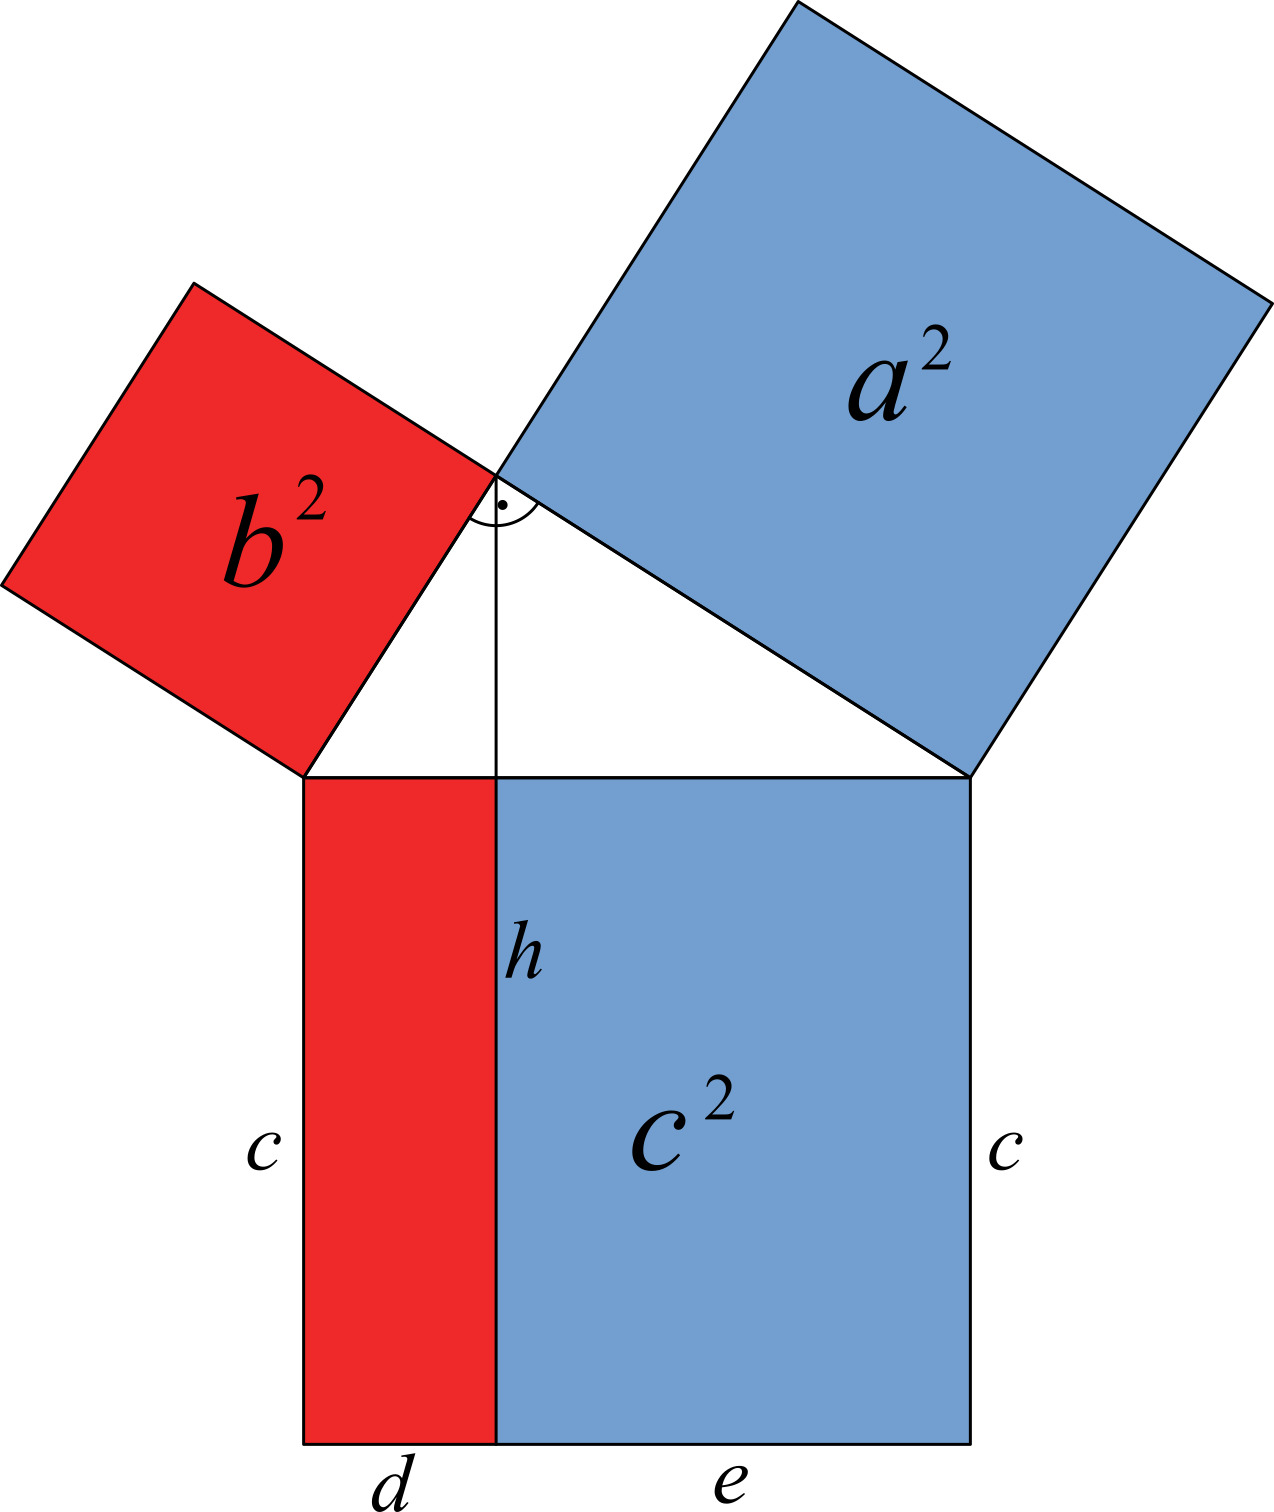
\includegraphics[width=50mm]{charly-pyth5.jpg}}}},{Beweis von Euklid}]

Das Ziel des Beweises ist es, zu zeigen, dass der Flächeninhalt von $a^2$ mit dem Flächeninhalt von $b^2$ zusammen genauso groß ist wie der Flächeninhalt von $c^2$ \cite[Proof #1]{CutTheKnot} \cite{Euklid4}. Dafür wird das Dreieck in zwei Teile geteilt. Zu zeigen ist, dass der Flächeninhalt von $a^2$ dem Flächeninhalt von dem rechts neben der Höhe $h$ liegendem Rechteck in $c^2$ entspricht und $b^2$ dem Flächeninhalt von dem links neben der Höhe $h$ liegendem Rechteck in $c^2$ (siehe Abb. 3), also dass Folgendes gilt:

\vspace*{-0.75cm}
\hspace*{-1.3cm}
\begin{minipage}{10cm}
  \begin{flalign*}
    a^2 = c \cdot e \textrm{\quad und \quad} b^2 = c \cdot d.\\
  \end{flalign*}
\end{minipage}
\vspace*{-0.75cm}

\end{figwindow}

\begin{figwindow}[0,r,{\vbox{\vskip-1mm \hbox{\hskip10mm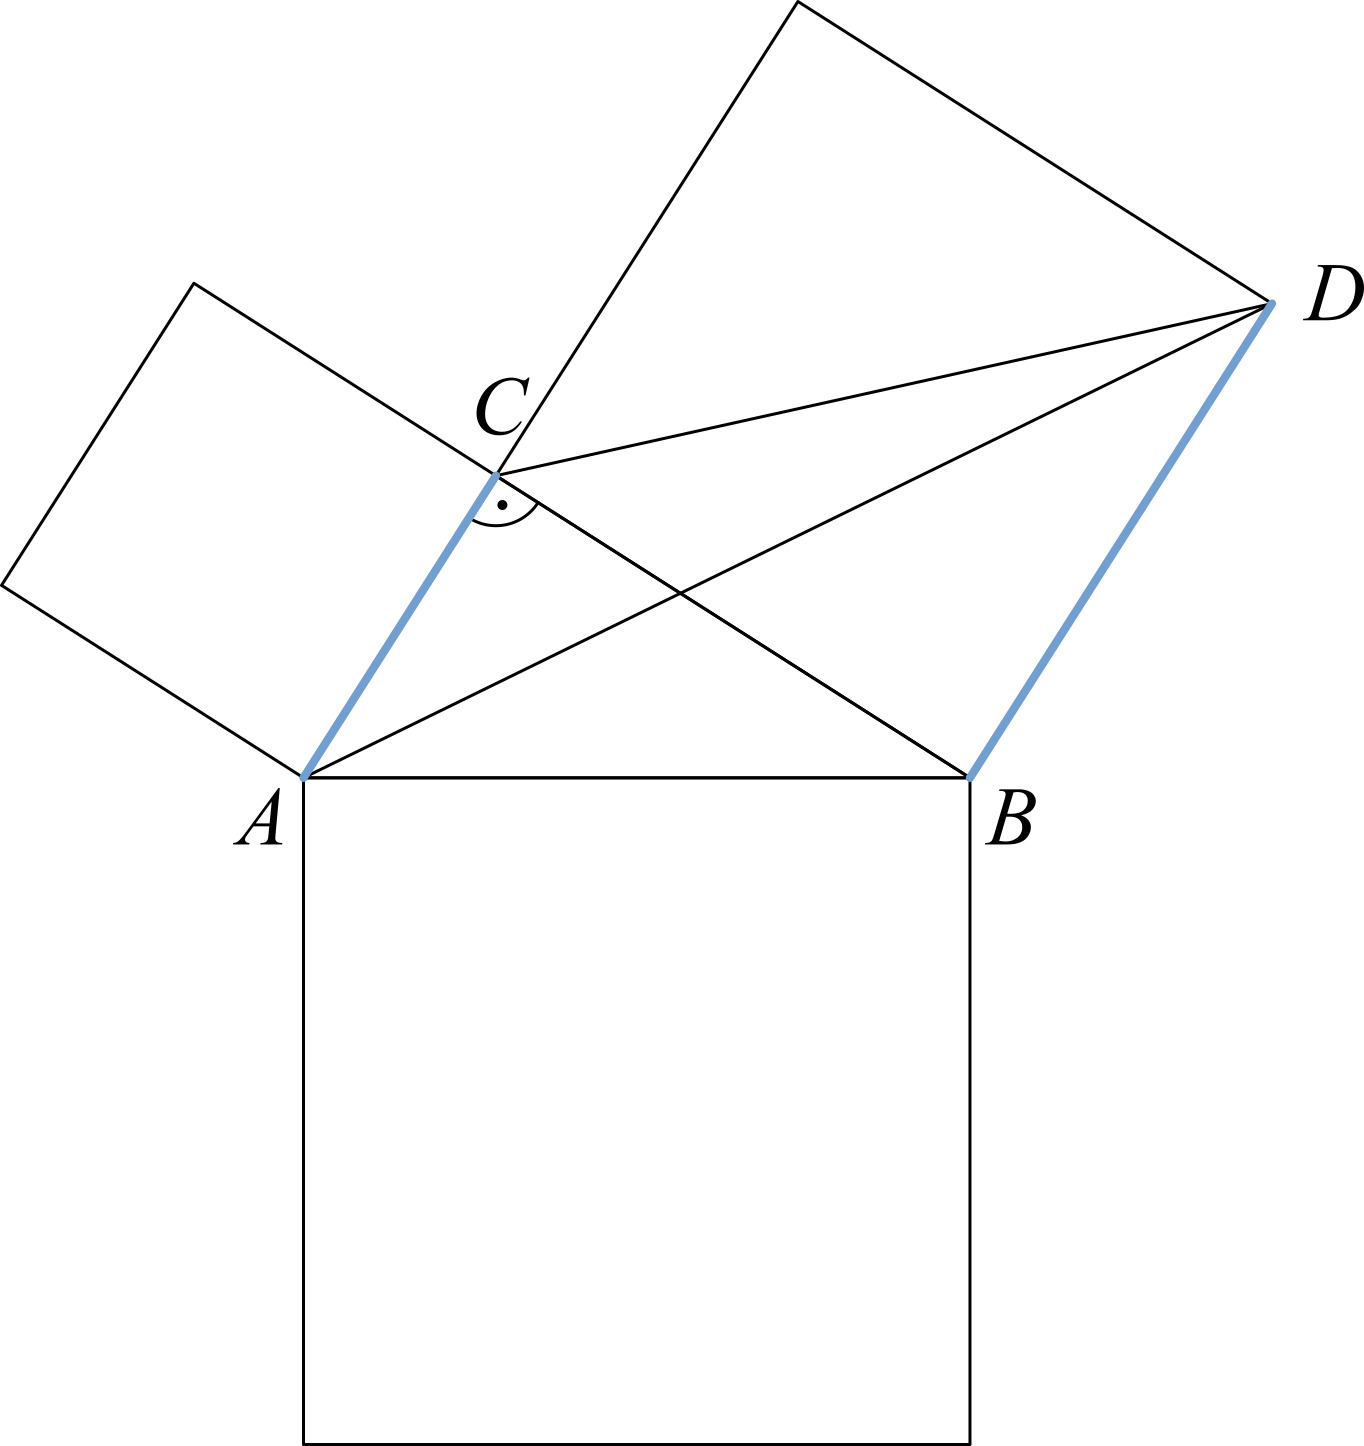
\includegraphics[width=60mm]{charly-pyth6.jpg}}}},{Beweis von Euklid}]

Zunächst wird das Dreieck $BDC$ (siehe Abb. 4) mit dem Flächeninhalt

\vspace*{-0.75cm}
\hspace*{-1.3cm}
\begin{minipage}{10cm}
  \begin{flalign*}
    A_{BDC} = \frac{1}{2} \cdot a^2\\
  \end{flalign*}
\end{minipage}
\vspace*{-0.75cm}

an der Strecke $\overline{AC}$ geschert (siehe Anhang 5.2) und es entsteht das Dreieck $ABD$. Da $\overline{AC} \parallel \overline{BD}$, gilt:

\vspace*{-0.75cm}
\hspace*{-1.3cm}
\begin{minipage}{10cm}
  \begin{flalign*}
    A_{BDC} = A_{ABD}.\\
  \end{flalign*}
\end{minipage}
\vspace*{-0.75cm}

\end{figwindow}

\begin{figwindow}[0,r,{\vbox{\vskip-1mm \hbox{\hskip10mm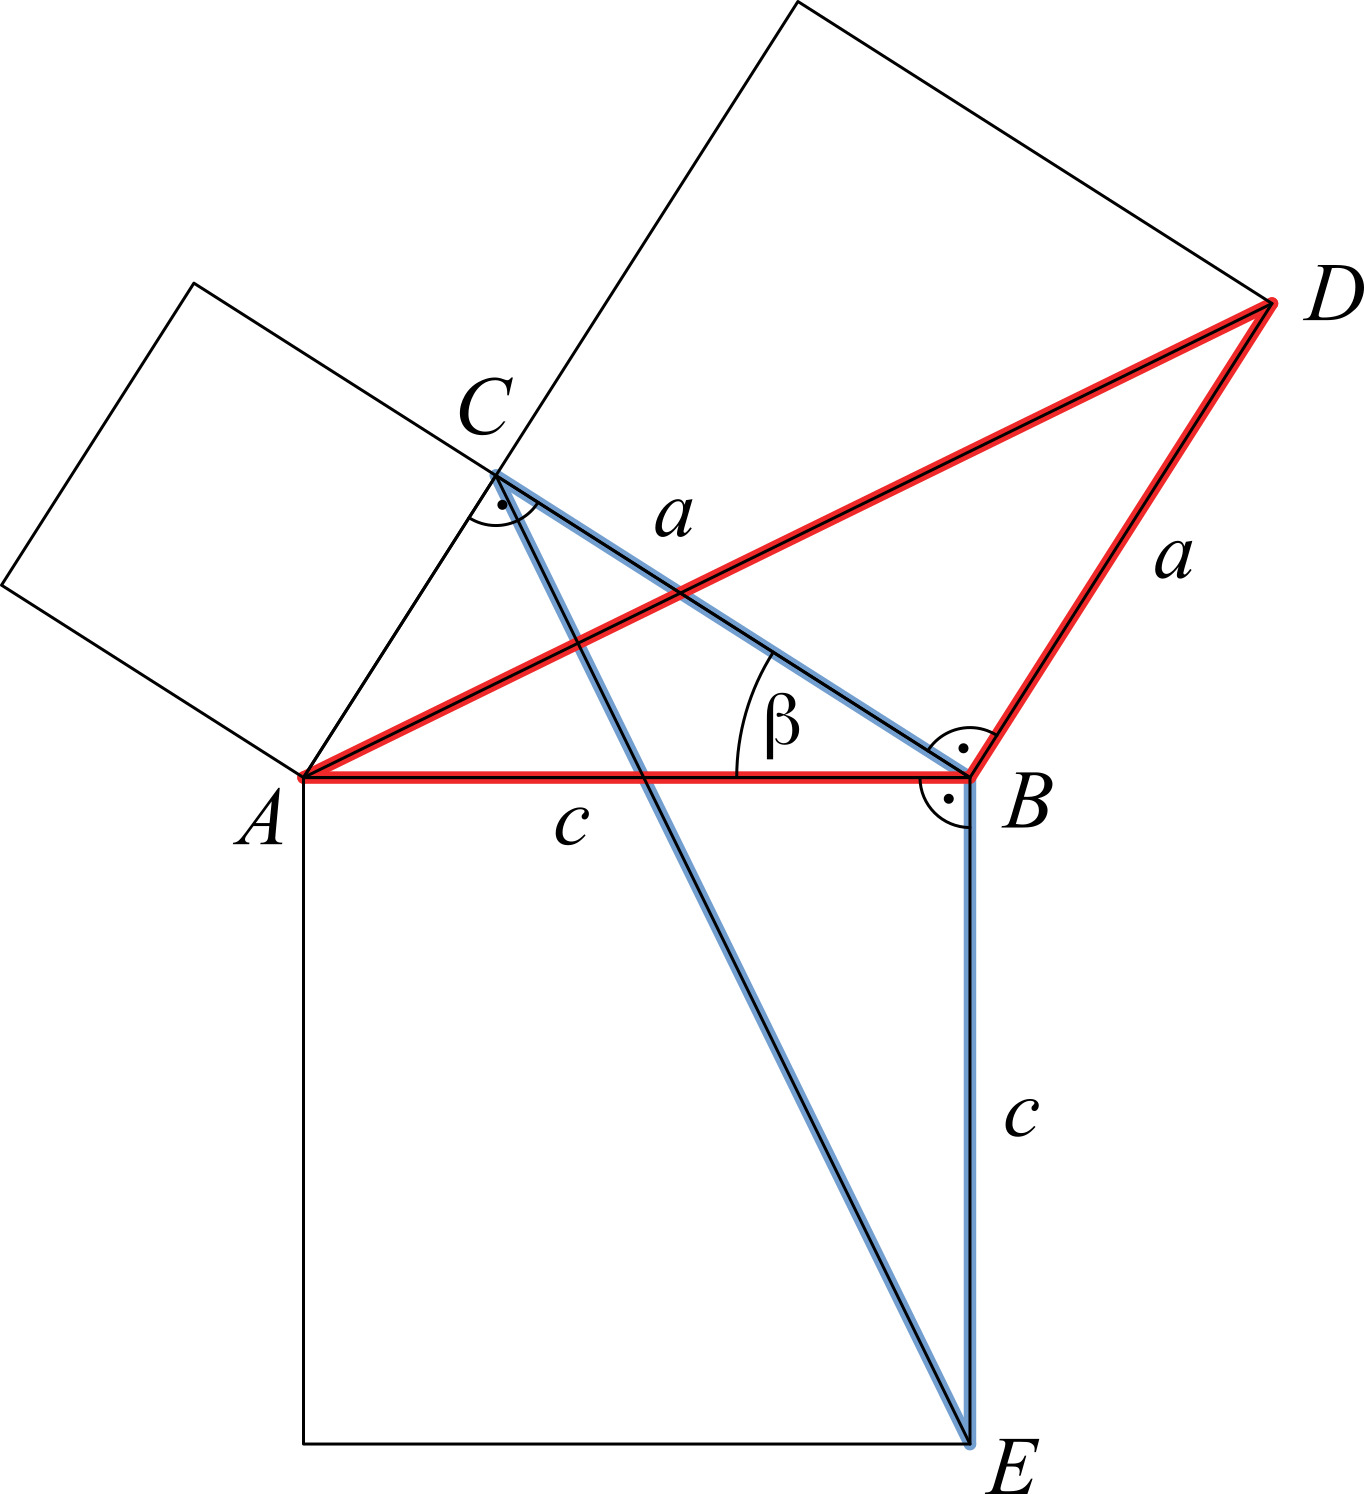
\includegraphics[width=50mm]{charly-pyth7.jpg}}}},{Beweis von Euklid}]

Nach dem Kongruenzsatz SWS sind die beiden Dreiecke $ABD$ und $BCE$ kongruent, da sie beide eine Seite der Länge $a$ und eine Seite der Länge $c$ haben und der Winkel zwischen den Seiten $a$ und $c$ bei beiden Dreiecken $90^\circ + \beta$ beträgt (siehe Abb. 5). Wenn man also das Dreieck $ABD$ um den Punkt $B$ um $90^\circ$ dreht, erhält man das Dreieck $BCE$, für das Folgendes gilt:

\end{figwindow}

\begin{figwindow}[0,r,{\vbox{\vskip-1mm \hbox{\hskip10mm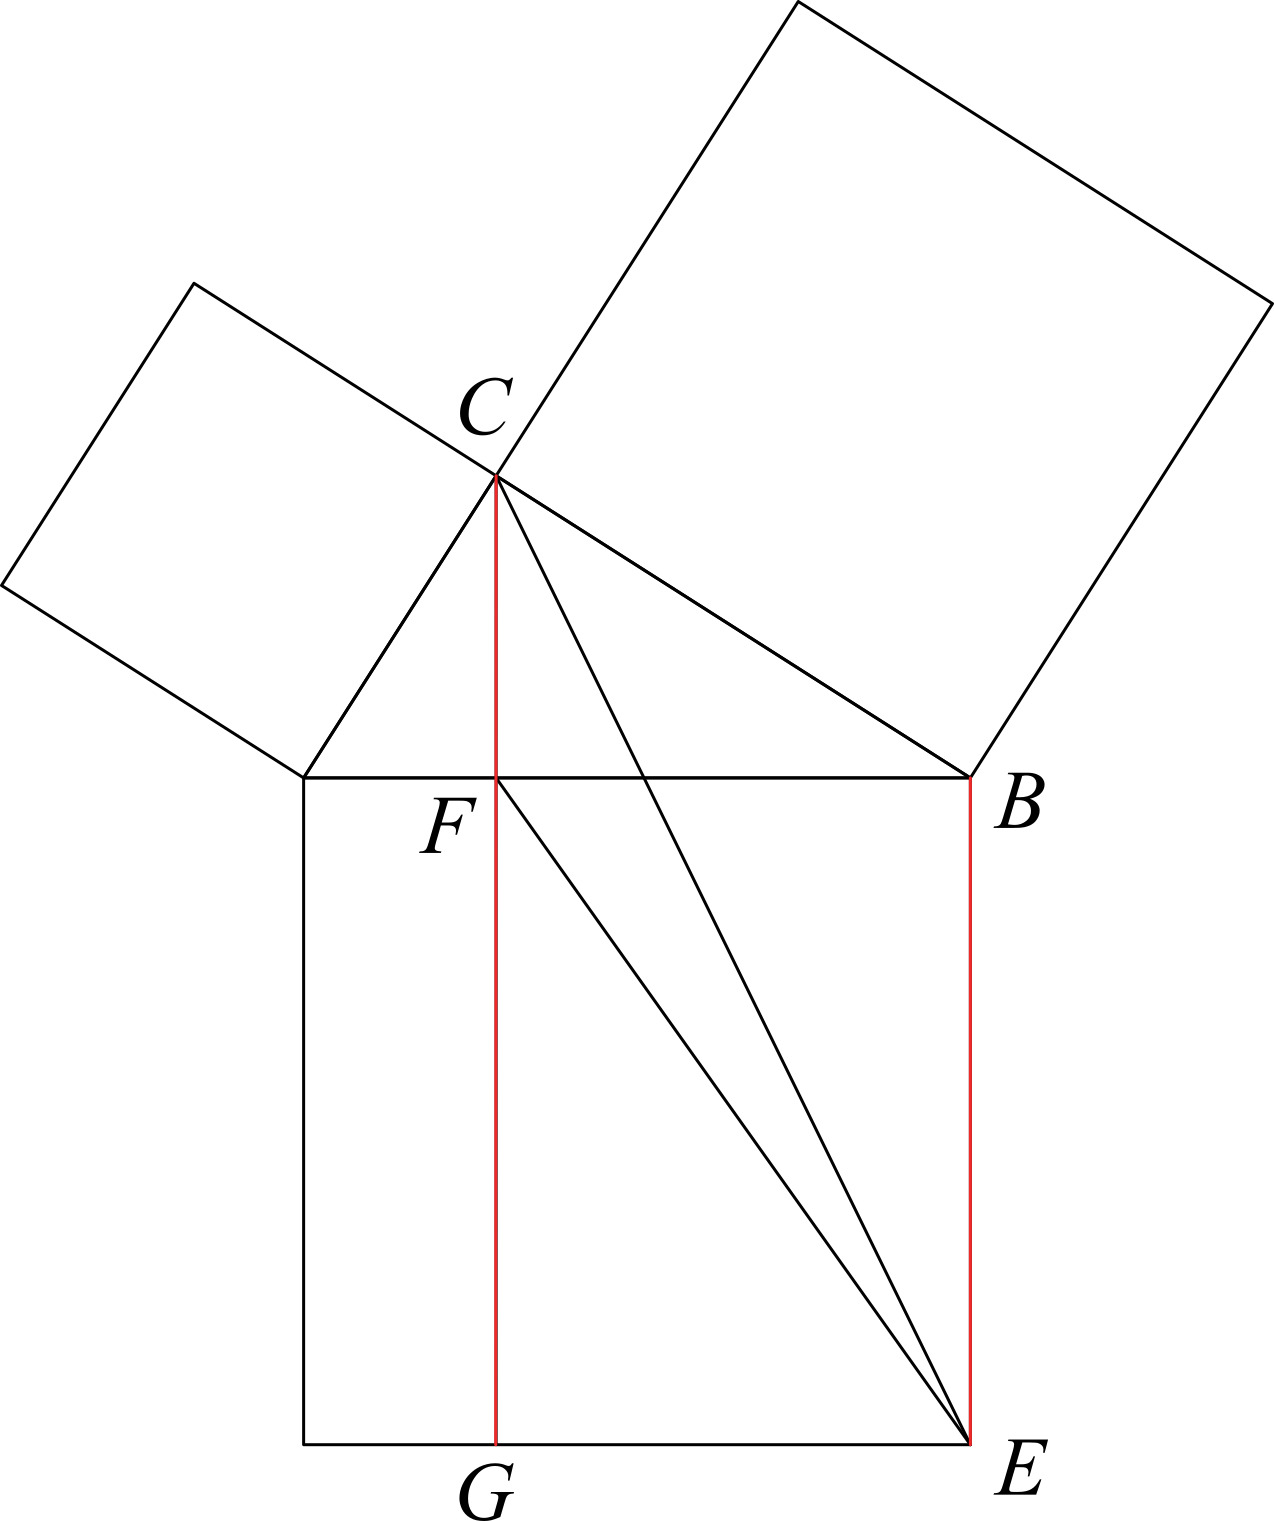
\includegraphics[width=50mm]{charly-pyth8.jpg}}}},{Beweis von Euklid}]

\vspace*{-0.75cm}
\hspace*{-1.3cm}
\begin{minipage}{10cm}
  \begin{flalign*}
    A_{ABD} = A_{BCE}.\\
  \end{flalign*}
\end{minipage}
\vspace*{-0.75cm}

Nun wird das Dreieck $BCE$ an der Strecke $\overline{CF}$ geschert und es entsteht das Dreieck $BFE$ (siehe Abb. 6). Da $\overline{CF} \parallel \overline{BE}$, gilt:

\vspace*{-0.75cm}
\hspace*{-1.3cm}
\begin{minipage}{10cm}
  \begin{flalign*}
    A_{BCE} = A_{BFE}.\\
  \end{flalign*}
\end{minipage}
\vspace*{-0.75cm}

\end{figwindow}

Also gilt:

\vspace*{-0.75cm}
\hspace*{1.5cm}
\begin{minipage}{10cm}
  \begin{flalign*}
    \frac{1}{2} a^2 = A_{BDC} = A_{ABD} = A_{BCE} = A_{BFE} = \frac{1}{2} \cdot c \cdot e \enspace \Rightarrow{} \enspace a^2 = c \cdot e.\\
  \end{flalign*}
\end{minipage}
\vspace*{-0.75cm}

Das Gleiche kann man für das Quadrat über der Seite $b$ wiederholen. Dann ergibt sich:

\vspace*{-0.75cm}
\hspace*{1.5cm}
\begin{minipage}{10cm}
  \begin{flalign*}
    b^2 = c \cdot d.\\
  \end{flalign*}
\end{minipage}
\vspace*{-0.75cm}

Wenn man die beiden Gleichungen addiert, ergibt sich mit $d + e = c$:
\begin{comment}
\vspace*{-0.75cm}
\hspace*{1.5cm}
\begin{minipage}{10cm}
  \begin{flalign*}
    a^2 + b^2 = c \cdot e + c \cdot d,\\
    a^2 + b^2 = c \cdot (d + e),\\
    a^2 + b^2 = c^2. \quad\Box\\
  \end{flalign*}
\end{minipage}
\vspace*{-0.75cm}
\end{comment}
\begin{align*}
a^2 + b^2 &= c \cdot e + c \cdot d, \\
          &= c \cdot (e + d), \\
          &= c^2. \quad\Box
\end{align*}
\subsection{Beweis von da Vinci}

Leonardo da Vinci (1452--1519 \cite{DaVinciGeschichte}) war ein berühmter italienischer Universalgelehrter. Er beschäftigte sich unter anderem mit Anatomie, Malerei, Architektur, Philosophie und Mathematik. Für den Satz des Pythagoras fand er den folgenden Beweis \cite{DaVinciBeweis}.

\begin{figwindow}[0,r,{\vbox{\vskip-1mm \hbox{\hskip10mm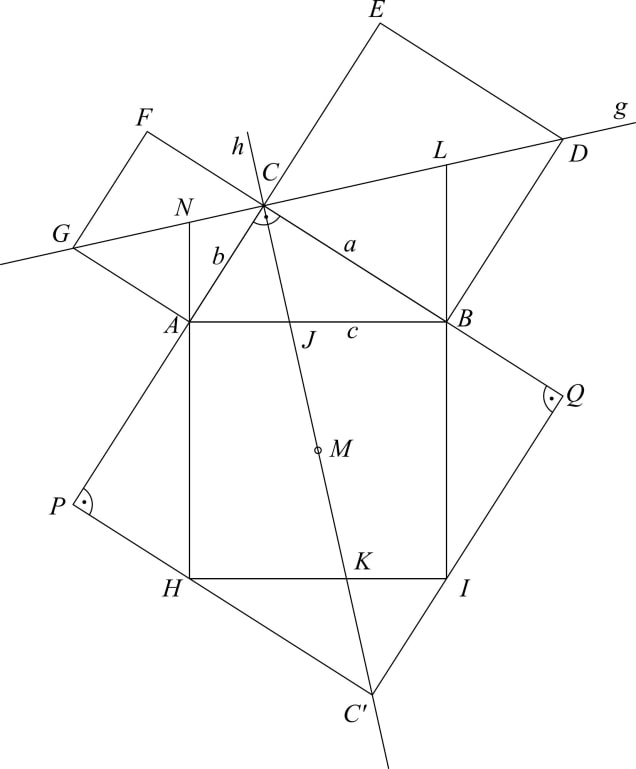
\includegraphics[width=70mm]{ charly-DaVinci1-the-original-best.jpg}}}},{Beweis von da Vinci}]

In Abbildung 7 ist ein rechtwinkliges Dreieck $ABC$ zu sehen. An die drei Seiten ist jeweils ein Quadrat angelegt. An dem Hypotenusenquadrat wird das Dreieck $ABC$ gespiegelt. Außerdem werden die zum Dreieck $ABC$ kongruenten Dreiecke $PHA$ und $IQB$ angelegt, sodass das Quadrat $C'QCP$ entsteht. Es gilt also:

\vspace*{-0.75cm}
\hspace*{-1.1cm}
\begin{minipage}{10cm}
  \begin{flalign*}
    \hspace*{-14mm} (\textrm{\rom{1}}) \quad A_{ABC} = A_{HC'I} = A_{PHA} = A_{IQB}.\\
  \end{flalign*}
\end{minipage}
\vspace*{-0.75cm}

(\rom{2}) Die Gerade $g$ schneidet die Punkte $G$, $C$ und $D$ und halbiert so die beiden Kathetenquadrate. \\Also gilt $\angle AGN = \angle NGF = \angle EDL = \angle LDB = 45^\circ$.

\end{figwindow}

(\rom{3}) Die Gerade $h$ schneidet die Punkte $C$, $M$ und $C'$, wobei $M$ der Mittelpunkt des Quadrats $AHIB$ ist.

(\rom{4}) Weiterhin ergibt sich, dass $h$ das Quadrat $C'QCP$ halbiert und somit $\angle ACC' = \angle C'CB = \angle CC'H = \angle IC'C = 45^\circ$ gilt.

Aus (\rom{4}) ergibt sich, dass die Vierecke $CAHC'$ und $C'IBC$ kongruent sind und somit Folgendes gilt:

\vspace*{-0.75cm}
\hspace*{1.5cm}
\begin{minipage}{10cm}
  \begin{flalign*}
     (\textrm{\rom{5}}) \quad A_{CAHC'} = A_{C'IBC}.\\
  \end{flalign*}
\end{minipage}
\vspace*{-0.75cm}

\begin{figwindow}[0,r,{\vbox{\vskip-1mm \hbox{\hskip10mm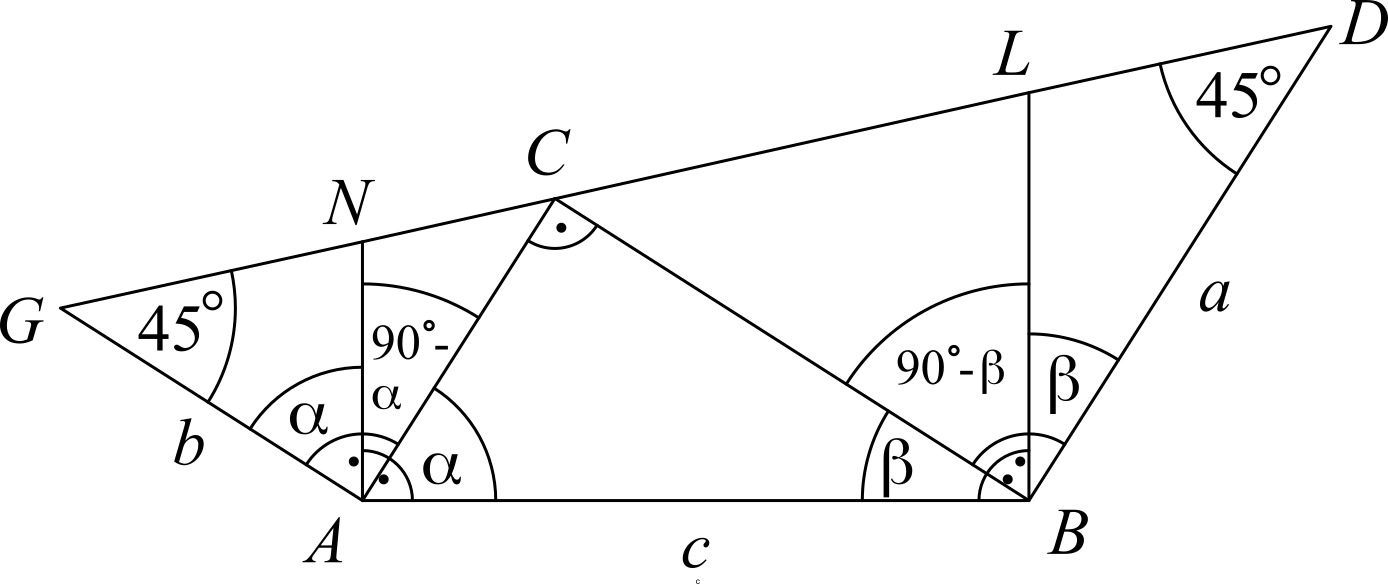
\includegraphics[width=80mm]{ charly-DaVinci3.jpg}}}},{Beweis von da Vinci}]

Die beiden Vierecke $GABD$ (siehe Abb. 8) und $CAHC'$ (siehe Abb. 9) sind aus der Abbildung 7 entnommen.

Diese beiden Vierecke sind kongruent. Um diese Aussage zu belegen, werden die Vierecke je in zwei Dreiecke $ANG$  bzw. $AJC$ und $BDL$ bzw. $C'KH$ und ein Trapez $ABLN$ bzw. $AHKJ$ geteilt.

\end{figwindow}

\begin{figwindow}[0,r,{\vbox{\vskip-1mm \hbox{\hskip10mm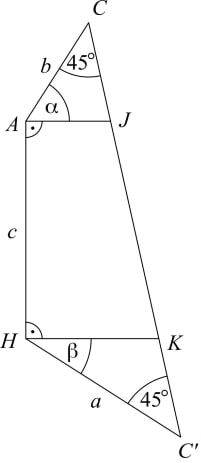
\includegraphics[width=40mm]{ charly-DaVinci2.jpg}}}},{Beweis von da Vinci}]

Die beiden Dreiecke $ANG$ und $AJC$ sind nach dem Kongruenzsatz WSW kongruent, da sie beide eine Seite mit der Länge $b$ haben, an der der Winkel $\alpha$ und ein $45^\circ$-Winkel (nach \rom{4} und \rom{2}) anliegen.

Die Dreiecke $BDL$ und $C'KH$ sind ebenfalls nach dem Kongruenzsatz WSW kongruent, da sie beide eine Seite mit der Länge $a$ haben, an der der Winkel $\beta$ und ein $45^\circ$-Winkel anliegt (nach \rom{4} und \rom{2}).

Die Trapeze $ABLN$ und $AHKJ$ haben gleiche Innenwinkel und sind damit einander ähnlich. Da sie die Seite $\overline{AB}$ bzw. $\overline{AH}$ mit der Länge $c$ gemeinsam haben, sind sie kongruent.

\end{figwindow}

Also sind die beiden Vierecke $GABD$ und $CAHC'$ kongruent.

\begin{align*}
(\textrm{\rom{6}}) \quad A_{CAHC'} &= A_{GABD}.
\end{align*}

Nun soll der Flächeninhalt des Vierecks $GABD$ (siehe Abb. 8) berechnet werden:
\begin{comment}
\vspace*{-0.75cm}
\hspace*{1.5cm}
\begin{minipage}{10cm}
  \begin{flalign*}
    A_{GAC} = \frac{1}{2} b^2 \textrm{ (nach } \rom{2}),\\
    A_{ABC} = \frac{1}{2} a b,\\
    A_{CBD} = \frac{1}{2} a^2 \textrm{ (nach } \rom{2}),\\
    A_{GABD} = A_{GAC} + A_{ABC} + A_{CBD}, \\
    = \frac{1}{2} b^2 + \frac{1}{2}ab + \frac{1}{2} a^2,\\
    = \frac{1}{2} \cdot (b^2 + ab + a^2).\\
  \end{flalign*}
\end{minipage}
\vspace*{-0.75cm}
\end{comment}
\begin{align*}
A_{GAC} &= \frac{1}{2} b^2 \quad\text{(nach \rom{2})},\\
A_{ABC} &= \frac{1}{2} a b,\\
A_{CBD} &= \frac{1}{2} a^2 \quad\text{(nach \rom{2})},\\
A_{GABD} &= A_{GAC} + A_{ABC} + A_{CBD} \\
&= \frac{1}{2} b^2 + \frac{1}{2}ab + \frac{1}{2} a^2\\
&= \frac{1}{2} \cdot (b^2 + ab + a^2).
\end{align*}
Nun soll der Flächeninhalt des Vierecks $CAHC'$ (siehe Abb. 9) berechnet werden. Zunächst wird der Flächeninhalt der Dreiecke berechnet. Da nach (\rom{1}) $A_{ABC} = A_{HC'I}$ gilt, gilt auch:

\begin{align*}
A_{\textrm{Dreiecke}} &= A_{AJC} + A_{HC'K} = \frac{1}{2}ab,\\
A_{AHKJ} &= \frac{1}{2}c^2 \quad\text{(nach \rom{4})},\\
A_{CAHC'} &= A_{\textrm{Dreiecke}} + A_{AHKJ} = \frac{1}{2}ab + \frac{1}{2}c^2 = \frac{1}{2} \cdot (ab + c^2).
\end{align*}

Nach (\rom{6}) gilt:

\begin{align*}
A_{CAHC'} &= A_{GABD},\\
\frac{1}{2} \cdot (ab + c^2) &= \frac{1}{2} \cdot (b^2 + ab + a^2) \qquad\vert \cdot 2,\\
ab + c^2 &= b^2 + ab + a^2 \qquad\vert -ab,\\
c^2 &= b^2 + a^2. \quad\Box
\end{align*}

\subsection{Beweis von Bhãskara \rom{2}}

Bhãskara \rom{2} (1114--1185 \cite{BhaskaraGeschichte1}) war ein indischer Mathematiker, der sich jedoch auch mit Astronomie beschäftigte. Er schrieb das Buch \textit{Bīja-ganita}, indem er unter anderem den folgenden Beweis für den Satz des Pythagoras veröffentlichte \cite{BhaskaraGeschichte2}.

\begin{figwindow}[0,r,{\vbox{\vskip-1mm \hbox{\hskip5mm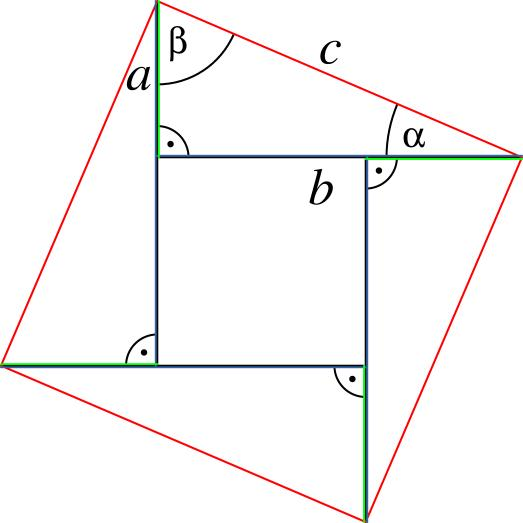
\includegraphics[width=60mm]{Bhaskaras1.jpg}}}},{Beweis von Bhãskara}]

Zunächst nahm er sich ein rechtwinkliges Dreieck mit den beiden Katheten $a$ und $b$ und der Hypotenuse $c$ \cite{BhaskaraBeweis1} \cite{BhaskaraBeweis2}. Dann vervierfachte er das Dreieck und drehte die vier Dreiecke so, dass ein Quadrat entstand (siehe Abb. 10). Dies ist möglich, da bei einem Dreieck die Innenwinkelsumme $180^\circ$ beträgt. Bei einem rechtwinkligen Dreieck muss deshalb $\alpha + \beta = 90^\circ$ gelten. Da immer die beiden Winkel $\alpha$ und $\beta$ die Ecken des Quadrats bilden und die Seitenlänge an jeder Kante $c$ beträgt,\\ entsteht ein Quadrat mit dem Flächeninhalt $c^2$.

\end{figwindow}

\begin{figwindow}[0,r,{\vbox{\vskip-1mm \hbox{\hskip10mm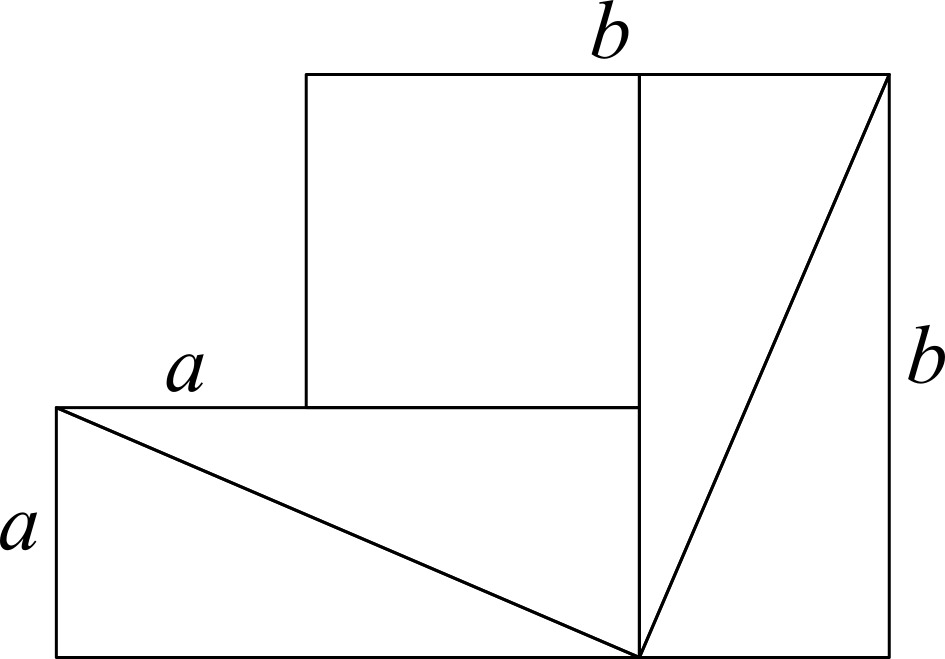
\includegraphics[width=60mm]{charly-Bhaskaras4.jpg}}}},{Beweis von Bhãskara}]

Wenn man nun das Dreieck rechts oben nach unten links verschiebt, bildet es genau ein Rechteck, da alle Dreiecke gleichgroß sind. Das gleiche kann man für das Dreieck links oben wiederholen und es entsteht ein weiteres Rechteck (siehe Abb. 11).

\end{figwindow}

\begin{figwindow}[0,r,{\vbox{\vskip-1mm \hbox{\hskip10mm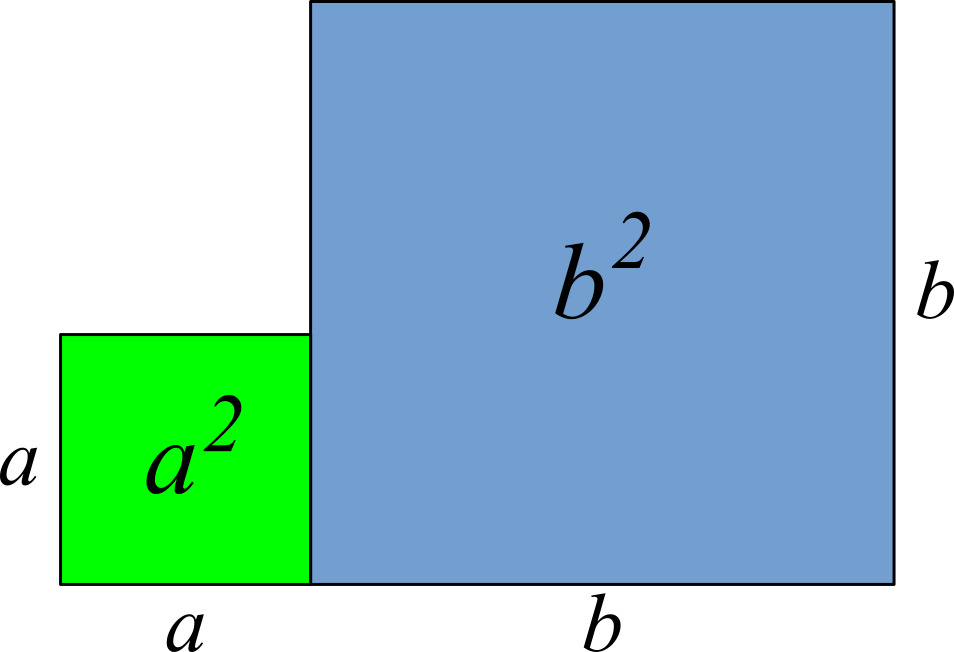
\includegraphics[width=60mm]{Bhaskara3.jpg}}}},{Beweis von Bhãskara}]

Nun entsteht eine Figur, die man in zwei Quadrate aufteilen kann (siehe Abb. 12). Das linke Quadrat hat die Seitenlänge $a$ und das rechte Quadrat die Seitenlänge $b$. Da die beiden Quadrate aus dem Ausgangsquadrat entstanden sind und so der Flächeninhalt gleich geblieben ist, gilt:

\vspace*{-0.75cm}
\hspace*{-1.3cm}
\begin{minipage}{10cm}
  \begin{flalign*}
    c^2 = a^2 + b^2. \quad\Box
  \end{flalign*}
\end{minipage}
\vspace*{-0.75cm}

\end{figwindow}

\subsection{Beweis von Garfield}

\begin{figwindow}[0,r,{\vbox{\vskip-1mm \hbox{\hskip10mm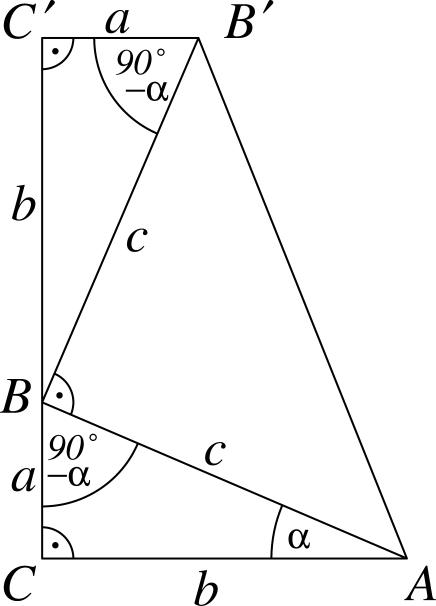
\includegraphics[width=40mm]{Garfield.jpg}}}},{Beweis von Garfield}]

Garfield (1831--1881 \cite{GarfieldGeschichte}) war der 20. Präsident der Vereinigten Staaten von Amerika, lieferte jedoch auch einen Beweis zum Satz des Pythagoras \cite{GarfieldBeweis1} \cite{GarfieldBeweis2}.

Gegeben ist ein rechtwinkliges Dreieck $ABC$, von dem eine Kopie $BB'C'$ um $-90^\circ$ gedreht an den Punkt $B$ angelegt wird. Die beiden Punkte $B'$ und $A$ werden verbunden (siehe Abb. 13).
\end{figwindow}

Um den Flächeninhalt des Trapezes $CAB'C'$ zu berechnen, kann man die Formel $A = m \cdot h$ benutzen, wobei $m$ die Länge der Mittellinie und $h$ die Höhe des Trapezes ist: 

\vspace*{-0.75cm}
\hspace*{1.5cm}
\begin{minipage}{10cm}
  \begin{flalign*}
    A_\text{Trapez} = \frac{a + b}{2} \cdot (a + b).\\
  \end{flalign*}
\end{minipage}
\vspace*{-0.75cm}

Man kann den Flächeninhalt des Trapezes aber auch als Summe der Flächeninhalte der Dreiecke beschreiben:

\vspace*{-0.75cm}
\hspace*{1.5cm}
\begin{minipage}{10cm}
  \begin{flalign*}
    A_\text{Trapez} = 2 \cdot \frac{a \cdot b}{2} + \frac{c^2}{2}.\\
  \end{flalign*}
\end{minipage}
\vspace*{-0.75cm}

\clearpage

Da beide Gleichungen den Flächeninhalt derselben Fläche beschreiben, kann man die beiden Terme gleichsetzen:
\begin{comment}
\vspace*{-0.75cm}
\hspace*{1.5cm}
\begin{minipage}{10cm}
  %\begin{align*}
  \begin{flalign*}
    (a+b) \cdot \frac{a+b}{2} = 2 \cdot \frac{a \cdot b}{2} + \frac{c^2}{2},\\
    \frac{1}{2} \cdot (a+b)^2 = a \cdot b + \frac{c^2}{2} \vert \cdot 2,\\
    (a+b)^2 = 2ab + c^2,\\
    a^2 + 2ab + b^2 = 2ab + c^2 \vert -2ab,\\
    a^2 + b^2 = c^2. \quad\Box
  \end{flalign*}
  %\end{align*}
\end{minipage}
\vspace*{-0.75cm}
\end{comment}
\begin{align*}
\frac{a+b}{2} \cdot (a+b) &= 2 \cdot \frac{a \cdot b}{2} + \frac{c^2}{2},\\
\frac{1}{2} \cdot (a+b)^2 &= a \cdot b + \frac{c^2}{2} \qquad\vert \cdot 2,\\
(a+b)^2 &= 2ab + c^2,\\
a^2 + 2ab + b^2 &= 2ab + c^2 \qquad\vert -2ab,\\
a^2 + b^2 &= c^2. \quad\Box
\end{align*}

\newpage

\section{Pierre de Fermat}

\subsection{Fermats Leben}

\begin{figwindow}[0,r,{\vbox{\vskip2mm \hbox{\hskip10mm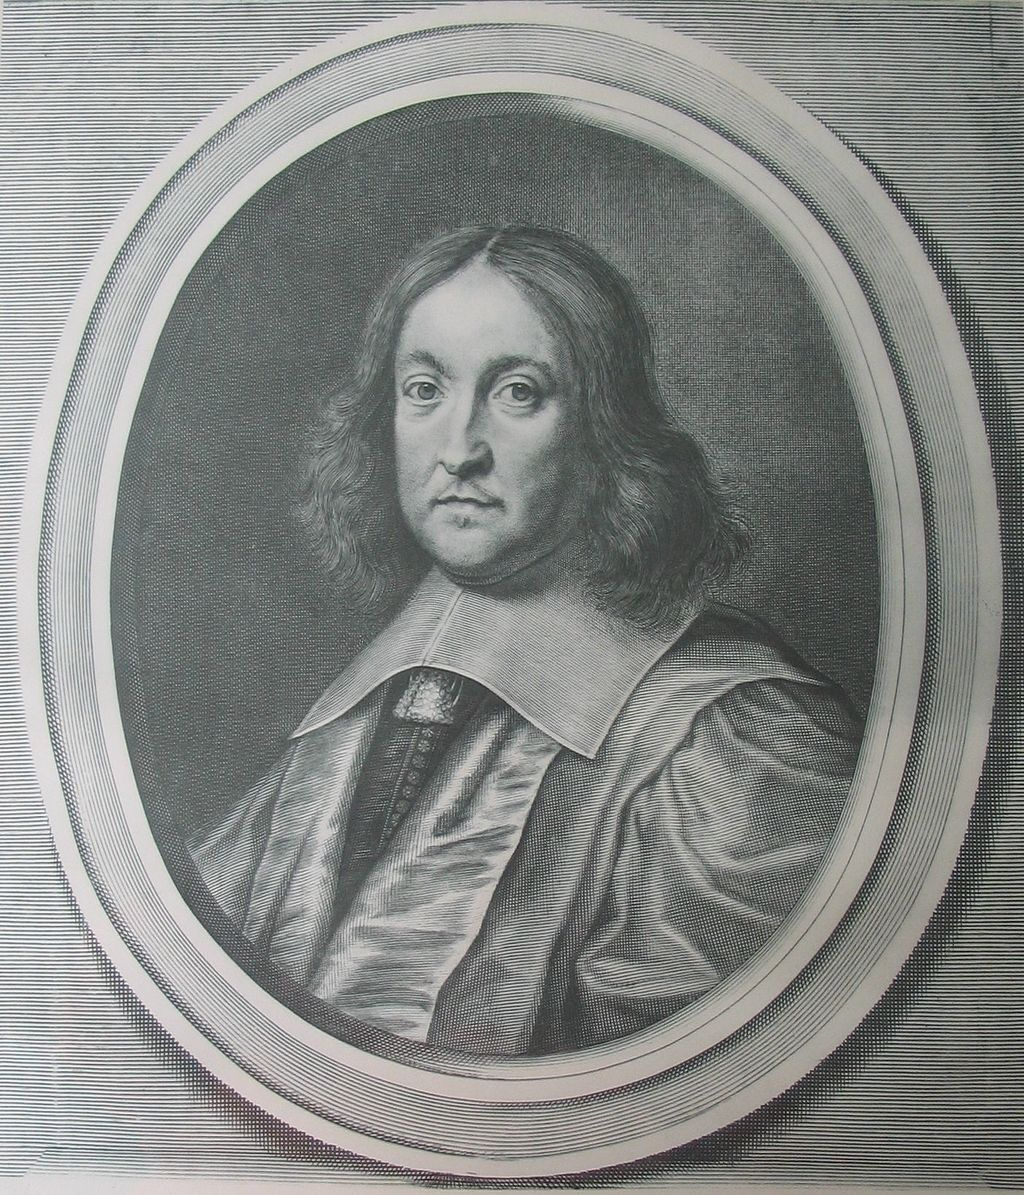
\includegraphics[width=50mm]{Fermat.jpg}}}},{Pierre de Fermat \cite{BildFermat}}]

Pierre de Fermat (siehe Abb. 14) war ein bedeutender französischer Mathematiker und Jurist. Er wurde 1607 \cite{FermatWiki} in Beaumont de Lomagne in Frankreich als Sohn des wohlhabenden und angesehenen Konsuls und Händlers Dominique Fermat und dessen Frau Françoise Cazeneuve Fermat geboren \cite{FermatsLeben} \cite[S. 59-65]{Buch}. Dort besuchte er wahrscheinlich das Collège de Navarre in Montauban und ging danach an die Universität in Toulouse. 1620 zog er nach Bordeaux, um dort seine mathematische Forschung zu betreiben. Danach studierte er von 1623 bis 1626 an der Universität in Orléans Zivilrecht \cite{FermatsLebenundSatz} und arbeitete ab 1626 als Anwalt in Bordeaux. Durch den Tod seines Vaters 1628 erbte Fermat sehr viel Geld und konnte es sich 1631 leisten, für 43 500 Livres Anwalt und Beamter in Toulouse zu sein. Durch dieses Amt bekam er mehr politische Rechte und stieg in den Amtsadel auf, weshalb er sich ab diesem Zeitpunkt Pierre \textit{de} Fermat nennen durfte. Im gleichen Jahr heiratete er Louise de Long und bekam später mit ihr acht Kinder.

\end{figwindow}

1636 begann sein Briefwechsel mit dem Mathematiker Marin Mersenne, mit dem er sich über mathematische Probleme austauschte. Oft hatte Fermat einen neuen Satz entdeckt und bat andere Mathematiker, ihm zu helfen einen Beweis zu finden, dabei hatte er bereits einen gefunden. Fermat war es wahrscheinlich nicht besonders wichtig, ein angesehener Mathematiker zu sein, da er kaum Entdeckungen publizierte. Er hatte eher Spaß daran, neue Sätze zu entdecken und zu beweisen und per Brief andere Mathematiker mit sehr schwierigen Problemen herauszufordern.

1641 notierte er erstmals seine Vermutung, die heute ,,Der Große Fermatsche Satz'' genannt wird, auf die ich später noch genauer eingehen werden.

1652 stieg er in die höchste Ebene des Strafgerichts auf und wurde ein angesehener Richter. Ein Jahr später erkrankte er an der Pest und wurde schon von seinem Freund Bernard Medon für tot erklärt, doch später stellte sich heraus, dass er durch seine gute medizinische Versorgung überlebte und sich wieder nahezu erholte.

Neben seiner juristischen Arbeit beschäftigte sich Fermat in seiner Freizeit vor allem mit der Mathematik. So hat er viel zur Entwicklung der Integral- und Differenzialrechnung beigetragen, aber auch zur Entwicklung der analytischen Geometrie, der algebraischen Geometrie und der Wahrscheinlichkeitsrechnung. Neben der Mathematik beschäftigte er sich mit physikalischen Themengebieten, wie der Berechnung der Masse der Erde und der Lichtbrechung, schrieb kurze Gedichte und viele Kommentare zu verschiedenster Literatur und lernte mehrere europäische Sprachen.

Am 12. Januar 1665 starb er in Castres.

\subsection{Der Große Fermatsche Satz}

Die Pythagoreer suchten ganze Zahlen, auf die der Satz des Pythagoras zutrifft. Man nennt diese Zahlen die \textit{pythagoreischen Tripel}. Ein Beispiel für ein pythagoreisches Tripel ist $(3, 4, 5)$, denn $3^2 + 4^2 = 9 + 16 = 25 = 5^2$. Ein anderes pythagoreisches Tripel ist $(5, 12, 13)$, denn $5^2 + 12^2 = 25 + 144 = 169 = 13^2$. Es gibt unendlich viele pythagoreische Tripel, die man, wie Platon später entdeckte, mit $(n^2 - 1, 2n, n^2 + 1)$ mit $n \in \mathbb{N}$ entdecken kann, jedoch gibt es auch noch weitere pythagoreische Tripel, die man nicht mit dieser Formel finden kann \cite{PythagoreischeZahlentripel}.

Fermat war nachweislich der Erste, der sich die Frage stellte, ob es auch pythagoreische Tripel für andere Exponenten gäbe, denn er schrieb in einer Notiz am Rand einer Ausgabe der \textit{Arithmetica}, die er sich in einer Bibliothek auslieh (siehe Anhang 5.1), er habe einen Beweis dafür, dass es für die folgende Gleichung keine ganzzahligen Lösungen gäbe  \cite{GroßerFermatscheSatzWiki} \cite[S. 85-87]{Buch}:

\vspace*{-0.75cm}
\hspace*{1.5cm}
\begin{minipage}{10cm}
  \begin{flalign*}
    a^n + b^n &= c^n \quad \text{mit} \quad n \in \mathbb{N}, n > 2 \quad \text{und} \quad a,b,c \neq 0.\\
  \end{flalign*}
\end{minipage}
\vspace*{-0.75cm}

Daraufhin versuchten viele Mathematiker:innen, Tripel, die die Gleichung erfüllen zu finden, doch es wurden nur Annäherungen gefunden, wie zum Beispiel:

\vspace*{-0.75cm}
\hspace*{1.5cm}
\begin{minipage}{10cm}
  \begin{flalign*}
    6^3 + 8^3 &= 216 + 512 = 728 = 729 - 1 = 9^3 - 1.\\
  \end{flalign*}
\end{minipage}
\vspace*{-0.75cm}

\subsection{Beweise für einzelne Fälle}
Das Problem ist ziemlich einfach zu verstehen, doch es ist sehr schwierig, für Fermats Vermutung einen Beweis zu finden. Auch hier benötigt man einen eindeutigen allgemeingültigen Beweis, doch zunächst versuchten verschiedene Mathematiker:innen die fermatsche Vermutung für bestimmte natürliche Zahlen $n$ zu beweisen.

Leonhard Euler fand im Jahr 1738 einen Beweis für $n = 4$ und im Jahr 1753 einen für $n = 3$  \cite{GroßerFermatscheSatzWiki}.

Daraufhin wurde entdeckt, dass es reicht, wenn man Beweise für $n = 4$ und für alle $n$, die Primzahlen größer als $2$ sind, findet, da jede natürliche Zahl, die größer als $2$ und keine Primzahl ist, durch vier oder durch eine andere Primzahl teilbar ist und so ein Vielfaches einer bewiesenen Zahl ist und keinen zusätzlichen Beweis benötigt. Das Problem dabei ist nur, dass es unendlich viele Primzahlen gibt. 

1825 erbrachten Peter Gustav Lejeune-Dirichlet und Andrien-Marie Legendre einen Beweis, dass die fermatsche Vermutung für $n = 5$ zutrifft \cite[S. 133 f.]{Buch}.

Sophie Germain entdeckte, dass $a^n + b^n \neq c^n$ für alle $n$ gilt, die Sophie-Germain-Primzahlen sind. Das sind Primzahlen p für die gilt, dass $2p + 1$ auch eine Primzahl ist.

Legendre erweiterte Germains Beweis, indem er zeigte, dass die fermatsche Vermutung auch für alle Exponenten $n$ gilt, die eine Primzahl $p$ sind, auf die zutrifft, dass $k \cdot p + 1$ mit $k = 4, 8, 10, 14, 16$ auch eine Primzahl ist. Außerdem lieferte er 1832 einen weiteren Beweis für $n = 14$.

1839 zeigte Gabriel Lamé, dass die Vermutung auch für $n = 7$ gilt und 1885 wurde der Satz von G. B. Matthews für $n=11$ und $n=17$ bewiesen. J. Fell stellte 1943 eine Methode vor, um die fermatschen Vermutung für $n = 11$, $n = 17$ und $n = 23$ zu beweisen.

Cauchy und Lamé dachten, dass sie einen endgültigen Beweis gefunden hätten, doch Ernst Kummer wies sie auf einen Fehler in ihren Überlegungen hin. Sie haben für ihren Beweis Zahlen in Primfaktoren zerlegt, jedoch haben sie übersehen, dass man die Zahlen darüber hinaus auch als Produkt zweier komplexer Zahlen schreiben kann, wie man an dem folgenden Beispiel erkennen kann:

\vspace*{-0.75cm}
\hspace*{1.5cm}
\begin{minipage}{10cm}
  \begin{flalign*}
    2 \cdot 2 \cdot 2 \cdot 2 = 16,\\
    (1 + \sqrt{-15}) \cdot (1 - \sqrt{-15}) = 1^2 + 15 = 16. \\
  \end{flalign*}
\end{minipage}
\vspace*{-0.75cm}

1850 bewies Ernst Kummer den Satz für alle regulären Primzahlen. Es mussten also nur noch Beweise für irreguläre Primzahlen gefunden werden, von denen es zwar unendlich viele gibt, doch mithilfe von Computer konnte man später schnell die fermatsche Vermutung für alle $n < 10\mkmmm000$ und später für alle $n < 4\mkmmm000\mkmmm000$ beweisen \cite[S. 191]{Buch}.

Durch immer mehr Beweise wurde es mit der Zeit wahrscheinlicher, dass Fermats Vermutung stimmt, doch bis 1993 gab es keinen Beweis für alle $n > 2$.

\subsection{Die Taniyama-Shimura-Vermutung}

1955 wurde die Taniyama-Shimura-Vermutung erstmals von den beiden Mathematikern Yutaka Taniyama und Gorō Shimura veröffentlicht \cite{Taniyama-Shimura-Vermutung}. Sie besagt, dass es zwischen Modulformen und elliptischen Gleichungen den Zusammenhang gibt, dass es zu jeder $M$-Reihe einer Modulform eine passende $E$-Reihe einer elliptischen Gleichung gibt, die die gleichen Zahlenwerte beinhaltet \cite[S. 217]{Buch}.

Der Mathematiker André Weil war ebenfalls an der Vermutung beteiligt und versuchte zu untersuchen, ob alle elliptischen Gleichungen modular sind. Um Brücken zwischen diesen beiden mathematischen Gebieten aufzubauen, musste die Vermutung noch bewiesen und ein Muster erkannt werden, wie man zu einer $M$-Reihe die passende $E$-Reihe findet bzw.\ umgekehrt \cite[S. 223]{Buch}. 

1984 zeigt Gerhard Frey bei einer internationalen Mathematiker-Tagung in Paris, dass man, wenn man die Taniyama-Shimura-Vermutung beweist, gleichzeitig auch die fermatsche Vermutung bewiesen hat. Frey ist dabei jedoch ein Fehler unterlaufen, doch der Mathematiker Ken Ribet konnte kurz darauf zeigen, dass Frey trotzdem Recht hatte \cite[S. 228-235]{Buch}.

\subsection{Endgültiger Beweis von Andrew Wiles}

\begin{figwindow}[0,r,{\vbox{\vskip+3mm \hbox{\hskip10mm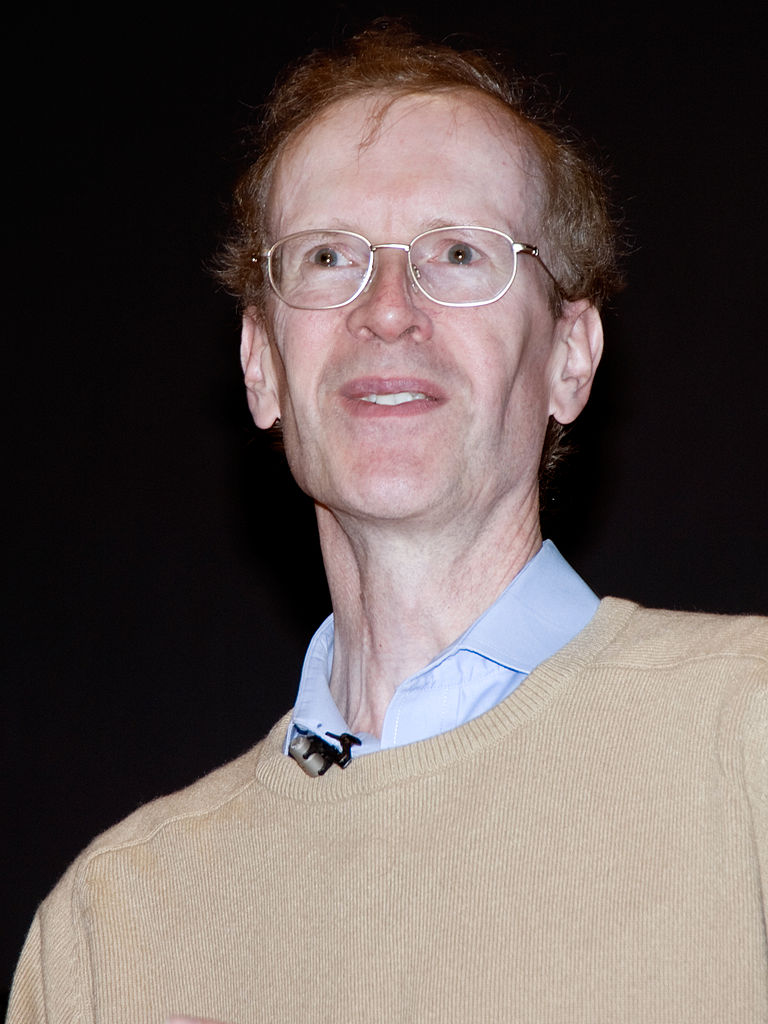
\includegraphics[width=60mm]{Wiles the real one.jpg}}}},{Andrew Wiles \cite{BildWiles}}]

Daraufhin begann der Mathematiker Andrew Wiles (siehe Abb. 15) mit seiner siebenjährigen Arbeit an einem Beweis der Taniyama-Shimura-Vermutung \cite[S. 237]{Buch}. 

Für seinen Beweis nutze er die Technik der vollständigen Induktion. Dafür musste er zunächst die Taniyama-Shimura-Vermutung für eine konkrete Zahl $n$ beweisen. Danach musste er zeigen, dass die Vermutung auch für $n + 1$ gilt. So gilt die Vermutung dann für alle natürlichen Zahlen bis ins Unendliche \cite[S. 243 f.]{Buch}. 
Andrew Wiles fiel auf, dass man die elliptischen Gleichungen in Familien einteilen kann. So konnte er dann die Taniyama-Shimura Vermutung für immer mehr Familien beweisen. 

Als er seinen Beweis beendet hatte, stellte er ihn in drei Vorträgen vom 21. bis zum 23. Juni 1993 auf einer Konferenz in Cambridge vor. Beim Prüfen seines Beweises wurde jedoch ein Fehler gefunden, doch gemeinsam mit seinem ehemaligen Studenten Richard Taylor konnte er den Fehler beheben, und so war nach 350 Jahren die fermatsche Vermutung bewiesen.

\end{figwindow}

1906 starb Paul Friedrich Wolfskehl, der sich leidenschaftlich mit der Suche nach einem Beweis beschäftigte, doch keinen fand. In seinem Testament vererbte er $100\mkmmm000$ Goldmark an die erste Person, die einen Beweis für alle $n>2$ findet. Diesen Wolfskehl-Preis erhielt Andrew Wiles  \cite{WolfskehlPreis}.

Ob Fermat wirklich schon einen Beweis hatte, ist nicht ganz sicher. Möglicherweise hatte er einen anderen und viel einfacheren Beweis, denn die von Wiles benutzten Methoden sind erst in den letzten Jahrhunderten, nach Fermats Tod,  entstanden. Es ist jedoch wahrscheinlicher, dass Fermat dachte, dass er einen Beweis hätte, doch ihm erst später auffiel, dass seine Überlegung einen Fehler hatte. Da er nicht die Absicht hatte, seine Notizen zu veröffentlichen, hat er seinen Fehler nicht mehr korrigiert. Die insgesamt 48 Bemerkungen am Rand der \textit{Arithmetika} wurden jedoch nach seinem Tod von seinem Sohn als Neuauflage veröffentlicht.

\newpage

\section{Anhang}

\subsection{Zitat: Fermats Kommentar}

Original: “Cubum autem in duos cubos, aut quadratoquadratum in duos quadratoquadratos, et generaliter nullam in infinitum ultra quadratum potestatem in duas ejusdem nominis fas est dividere: cujus rei demonstrationem mirabilem sane detexi. Hanc marginis exiguitas non caperet.”

Deutsche Übersetzung: „Es ist jedoch nicht möglich, einen Kubus in 2 Kuben, oder ein Biquadrat in 2 Biquadrate und allgemein eine Potenz, höher als die zweite, in 2 Potenzen mit ebendemselben Exponenten zu zerlegen: Ich habe hierfür einen wahrhaft wunderbaren Beweis entdeckt, doch ist dieser Rand hier zu schmal, um ihn zu fassen.“ \cite{GroßerFermatscheSatzWiki}

\subsection{Dreiecke scheren}

\begin{figwindow}[0,r,{\vbox{\vskip-1mm 
\hbox{\hskip10mm\includegraphics[width=60mm]{Dreieckescheren.jpg}}}},{Dreiecke scheren}]

Wenn man die Spitze eines Dreiecks auf einer Geraden, die parallel zur Grundlinie des Dreiecks verläuft, verschiebt, bleibt die Länge der Grundlinie $g$ und die Höhe $h$ gleichgroß. Da $A = \frac{1}{2}\cdot g \cdot h$ gilt, bleibt der Flächeninhalt des Dreiecks gleich groß.

\end{figwindow}

\newpage

\subsection{Vollkommene, abundante und defiziente Zahlen}

Eine Zahl ist {\em abundant}, wenn die Summe ihrer Teiler größer als die Zahl selbst ist. Ein Beispiel für eine abundante Zahl ist die $12$, denn wenn man ihre Teiler addiert, ist die Summe  $1 + 2 + 3 + 4 + 6 = 16$ größer als $12$.

Eine Zahl ist {\em vollkommen}, wenn die Summe ihrer Teiler genauso groß ist, wie die Zahl selbst. Ein Beispiel für eine vollkommene Zahl ist die $6$, denn wenn man ihre Teiler addiert, ist die Summe  $1 + 2 + 3 = 6$ genauso groß wie die $6$. Diese vollkommenen Zahlen kann man finden, indem man in die Formel $(2^n-1) \cdot 2^{n-1}$ eine natürliche Zahl einsetzt, so dass $(2^n)-1$ eine Primzahl wird (Mersenne'schen Primzahl) \cite{VollkommeneZahlenFinden}.

Eine Zahl ist {\em defizient}, wenn die Summe ihrer Teiler kleiner als die Zahl selbst ist. Ein Beispiel für eine defiziente Zahl ist die $10$, denn wenn man ihre Teiler addiert, ist die Summe  $1 + 2 + 5 = 8$ kleiner als $10$ \cite[S. 34-37]{Buch}. 

\newpage
\newpage


%\setlength\bibitemsep{\baselineskip}

\printbibliography
\newpage
%%Nicht anfassen, so ist der Dokumentenaufbau
\addtocontents{toc}{\protect\setcounter{tocdepth}{0}}
\renewcommand{\appendixtocname}{Anhang}
\addappheadtotoc
\renewcommand{\appendixpagename}{Anhang}
\appendices
\appendixpage
\appendixtitleoff
%%%%%%%%%%%%%%%%%%%%%%%%%%%%%
%%%Ab hier Inhalt einfügen%%%
%%%%%%%%%%%%%%%%%%%%%%%%%%%%%



%%%%%%%%%%%%%%%%%%%%%%%%%%%%
%%%%%Ende des Dokuments%%%%%
%%%%%%%%%%%%%%%%%%%%%%%%%%%%
\MSonehalfspacing
\newpage
\restoreapp


\newpage
\section*{Eigenständigkeitserklärung}


Hiermit versichere ich, dass ich die BLL selbstständig verfasst und keine anderen als die angegebenen Quellen und Hilfsmittel benutzt habe, alle Ausführungen, die anderen Schriften wörtlich oder sinngemäß entnommen wurden, kenntlich gemacht sind und die Arbeit in gleicher oder ähnlicher Fassung noch nicht Bestandteil einer Studien- oder Prüfungsleistung war.

\noindent{}Berlin, den 4. Dezember 2021
\begin{minipage}[t]{8cm}
\centering \hspace{20mm} \hrulefill \\
\end{minipage}

\end{document}
